\documentclass{iitthesis}

%   \documentclass[draft]{iitthesis}

%\usepackage[dvips]{graphicx}    % This package is used for Figures
\usepackage{graphicx}    % This package is used for Figures
\usepackage{epstopdf}
\usepackage{placeins}
%\usepackage{rotating}           % This package is used for landscape mode.
\usepackage{epsfig}
\usepackage{subfigure}          % These two packages, epsfig and subfigure, are used for creating subplots.
\usepackage{mathtools}          % used for equations
\usepackage{listing}
\usepackage{xcolor}
\usepackage[final]{mcode}
% Packages are explained in the Help document.


\begin{document}
%%fakesection{TITLES AND INDEXES)
%%% Declarations for Title Page %%%
\title{Energy savings for UAV flight in unsteady gusting conditions \\
through trajectory optimization }
\author{Lou Grimaud}
\degree{Master of Science}
\dept{Mechanical, Materials, and Aerospace Engineering}
\date{July 2014}
%\copyrightnoticetrue      % crate copyright page or not
\maketitle                % create title and copyright pages


\prelimpages         % Settings of preliminary pages are done with \prelimpages command


%%%  Acknowledgement %%%
\begin{acknowledgement}     % acknowledgement environment, this is optional
  \par  This dissertation could not have been written without Dr. X
  who not only served as my supervisor but also encouraged and
  challenged me throughout my academic program. He and the other
  faculty members, Dr. Y and Dr. Z, guided me through the
  dissertation process, never accepting less than my best efforts. I
  thank them all.\\ \\ (Don't copy this sample text. Write your own
  acknowledgement.)
%\input{acknowledgement.tex} % you need a separate acknowledgement.tex file to include it.
\end{acknowledgement}


% Table of Contents
\tableofcontents
\clearpage

% List of Tables
\listoftables

\clearpage

%List of Figures
\listoffigures

\clearpage

%List of Symbols(optional)

\listofsymbols


\SymbolDefinition{$C_l$}{Lift coefficient}
\SymbolDefinition{$C_d$}{Drag coefficient}
\SymbolDefinition{$W_a$}{Non-dimensional gust amplitude}
\SymbolDefinition{$T_g$}{Non-dimensional gust duration}
\SymbolDefinition{$T$}{Vehicle time scale ($=\frac{V_cr}{g}$)}
\SymbolDefinition{$V_cr$}{Vehicle cruse speed}
\SymbolDefinition{$C_l^*, C_d^*$}{Lift and drag coefficients at the optimal lift to drag ratio}
\SymbolDefinition{$G$}{lift to drag ratio}
\SymbolDefinition{$G^*$}{optimal (maximal) lift to drag ratio}
\SymbolDefinition{$Q$}{Non-dimensional dynamic pressure}
\SymbolDefinition{$X, Z, U, W$}{Non-dimensional positions and velocities}
\SymbolDefinition{$v$}{Relative wind velocity to the vehicle}
\SymbolDefinition{$L', D'$}{Lift and drag forces}
\SymbolDefinition{$V^*$}{Optimal glide speed}
\SymbolDefinition{$\gamma$}{Angle of the vehicle trajectory to the horizon}
\SymbolDefinition{$U_g, W_g$}{Non-dimensional horizontal and vertical gust velocity components}
\SymbolDefinition{$x$}{State vector used for the optimizatiion}
\SymbolDefinition{$y_i$}{Vector of position and velocities at point $i$}
\SymbolDefinition{$C_l^{qs}$}{Quasi-steady lift coefficient}
\SymbolDefinition{$x_0$}{State variable x value for quasi-steady cases}
\SymbolDefinition{$k$}{Non-dimesional reduced frequency ($=\pi c \frac{f}{u}$)}
\SymbolDefinition{$t^+$}{Airfoil time scale ($=\frac{U}{c}$)}
\SymbolDefinition{$c$}{Airfoil chord}
\SymbolDefinition{$u$}{Free stream velocity}
%\SymbolDefinition{$$}{<++>}<++>
%\SymbolDefinition{$<++>$}{<++>}<++>
%\SymbolDefinition{$<++>$}{<++>}<++>
%\SymbolDefinition{$<++>$}{<++>}<++>
%\SymbolDefinition{$<++>$}{<++>}<++>
%\SymbolDefinition{$<++>$}{<++>}<++>
%
\clearpage

%%% END OF INDEXES %%%
%%%%%%%%%%%%%%%%%%%%%%%%%%%%%%%%%%%%%%%%%%%%%%%%%%%%%%%%%%%%%%%%%%%%%%%%%%%%%%%%%%%%%%%

%%% Abstract %%%
\begin{abstract}           % abstract environment, this is optional
  \par The purpose of this thesis is to show how micro unmanned aerial vehicles can extract energy from natural wind gusts and how this energy extraction is affected by the effects of unsteady aerodynamics.

\par The trajectory of a small UAV flying through wind gusts is simulated with a two degrees of freedom model.
The non-dimensional model is set to include vertical and horizontal gusts of varying amplitudes and durations.
From this model an optimization routine is performed in order to obtain the minimum gust amplitude needed to get a neutral energy trajectory.
With these results, it is shown that neutral energy flight is possible through gusts speeds only 10 to 30\% of the flying speed of the aircraft .
Analysis of the results shows that the lift coefficient has to be changed very rapidly in order to perform these maneuvers in short duration gusts. 
Moreover high lift values are often required. 

\par To achieve this kind of rapid changes in the lift and drag forces, fast variations of the angle of attack are needed.
The high lift values also requires high angles of attacks that are likely to cause separation of the flow over the airfoil.
These fast variations at high angle of attack are shown to cause unsteady non linear aerodynamic responses.
Traditional CFD simulations are far too computationally expensive to be implemented into the optimization routine.
To solve this issue a low order model based on a paper by Goman and Khrabrov \cite{GK} is developed and validated against experimental results.
This model produces accurate predictions of the lift and drag coefficients for a wide range of angles of attack and for different type of pitch inputs.

\par With this light model the influence of the unsteady aerodynamics on the energy extraction problem are highlighted.
The main difference with quasi-steady aerodynamics model was found to be for gusts at a reduced frequency faster than k of 0.07.
Around these values the potential performances are improved by introducing the unsteady model.
The trajectories obtained include more violent changes in angle of attacks in order to take full advantages of the unsteady effects.


  %you need a separate abstract.tex file to include it.
\end{abstract}


\textpages     % Settings of text-pages are done with \textpages command

% Chapters are created with \Chapter{title} command
\Chapter{INTRODUCTION}

\Section{Motivations} \label{subsec:dynsoar}

\Subsection{Trajectory optimization through wind gusts}
The main challenge for electric small size unmanned aerial vehicle is the autonomy.
Battery energy density is limited and can rapidly become an important part of the weight of vehicle.
Since most of the energy is used by the electric engine for propulsion optimizing the control laws and trajectory could have a dramatic effect on endurance. 
With the progress in autonomous control software, successful attempts have been made by Allen \cite{flight_test_soaring_NASA} and Edwards \cite{flight_test_soaring_NCU} to extract energy from natural updrafts.
These experiments have shown that a UAV can take advantage of localized vertical winds naturally produced by thermal convection.

\par However, within an urban environment, such as the one mini and micro-UAV aircrafts are designed for, the gust's velocity profile is vastly different. 
Wind blowing through a group of buildings produces turbulent conditions with both vertical and horizontal vortices.
The turbulence levels can reach speeds representing a significant portion of micro-UAV's glide speed. 
In flow fields such as this, the gusts encountered are both faster and arguably more complex than the ones due to thermal convection.

\par The lack of low-order models for the unsteady aerodynamic effects means that all of the studies on trajectory optimization have been based on quasi-steady models to compute the aerodynamic forces.
More computationally expensive models traditionally used for CFD are too impractical considering the thousands of function evaluations needed for such algorithm.
To solve this problem, a low-order model capturing the unsteady behavior of the flow over the aircraft is needed.
Additionally this model needs to be able to handle flow separation and airfoil stalling since the maneuvers required for energy extraction can be relatively violent and often involve high angle of attack.


\Subsection{Pitching airfoil model}
The difficulty is that the lift and drag behavior in such condition is time dependent and non-linear.
As such, finite element methods are often the only solution to get a good simulation of the lift and drag.
Such solutions are useful, since they provide a lot of information about the flow field itself, but the computation time required to get the lift and drag out of them is several orders of magnitude too long.

\par Another solution explored by Brunton \cite{brunton2008unsteady} is to perform linear approximations of the lift and drag behavior at different angles of attack.
These linear models can then be patched together to include the non-linear behaviors.
The appeal of this method is that the individual linear models can be easily analyzed using classical linear time invariant (LTI) system theory.
It is however still fairly complicated and requires an extensive experimental study to identify the system at each set angle of attack.

\par The model developed by Goman and Khrabrov allows for a low-order non linear model to capture the features of the lift coefficient over a very wide range of angle of attack, as well as for any arbitrary pitch profile.
One quasi-steady map of the lift and two time constants are all that is needed to get the full model.
So far it seems that the use of this model has been limited to the lift coefficient predictions, however for the trajectory optimization the drag coefficient is also needed.

\Section{Previous investigations}

\par As explained in the previous part \ref{subsec:dynsoar}, the bulk part of the research on trajectory optimization for small flying vehicles has been focused on either natural convection, such as the one glider pilots and some birds (Denny \cite{denny2009dynamic}) take advantage of in plains, or wind gradients, such the ones found close to the surface of the ocean.
The latter are often exploited by seabirds such as albatrosses.

\par Lissaman conducted a study for 3D trajectories in differently shaped wind gradients close to the ground \cite{lissaman2005wind} as well as 2D trajectories through sinusoidal wind gusts \cite{Lissaman2007neutral}. 
His optimization is performed on a non-dimensional set of equations \cite{chakrabarty2010flight} that has been reused in this study.
He also uses different kind of profiles for the wind gradient in order to represent more accurately real wind gradients.
The approach pioneered by Lissaman forms the basis of the following optimization study.

\par However these studies have all only used quasi-steady aerodynamic model.
Airfoil interactions with more complex gusts structures such as the ones produced by vortices shed by upstream obstacles have also been studied with CFD tools by Golubev \cite{golubev2010high} \cite{golubev2010parametric}.

\par Traditional low order models that try to circumvent the use of CFD are often based on Theodorsen's \cite{theodorsen} and Greenberg's \cite{green} derivations of the Navier-Stokes equations for potential flow.
However experimental study of flow separation for pitching airfoils was started even earlier by Katzmayr in 1922 \cite{katz}.

\Chapter{Energy extraction optimization} \label{ch:Eni_extraction}

\Section{2 DoF model}

\Subsection{Non-dimensional equations of motion}

\par The model chosen for this simulation is a simple two degree of freedom, two dimension, point mass model. 
The aircraft is assumed to be a glider to simplify the optimization routine. 
With such assumption the equations of motion in the ground reference frame is :

\begin{equation}
	\begin{array}[c]{c}
		\dot{x}= -L \cdot sin(\gamma) + D \cdot cos(\gamma) \\ 
		\dot{y}= L \cdot cos(\gamma) - D \cdot sin(\gamma) - m \cdot g
	\end{array}
	\label{eqn:eqm}
\end{equation}

% should I include a figure with the reference frame, and angle definition?

\par The lift and drag are defined are :

\begin{equation}
	\begin{array}[c]{c}
		L= \frac{1}{2} \rho V^2 C_l \\ 
		D= \frac{1}{2} \rho V^2 C_d
	\end{array}
	\label{eqn:Cl_def}
\end{equation}

\Subsection{Lift and drag models}

\Section{Optimization process, cost function and constraints}

\Subsection{General consideration on optimization}
% Get some stuff from the MM544 class

\Subsection{Cost function and constraints formulation}

\Section{Results}




\Chapter{Modelling of the Lift coefficient under unsteady pitching motion} \label{Ch:gkmodel}

\Section{The Goman and Khrabrov model}

\Subsection{Motivation}
In their 1994 paper entitled ``State-Space Representation of Aerodynamic Characteristics of an Aircraft at High Angle of Attack'' \cite{GK} Goman and Khrabrov introduce a new model for characterizing the lift and moment coefficients for slender delta wings.
Their goal was to study the stability of delta wing fighter jets where maneuverability is important, and to link it to physical fluid dynamic phenomenons such as vortex breakdown or flow separation.

\par The classical stability analysis method relies on a Taylor series expansion of the aerodynamic coefficients.
% maybe put an example here.
This linear representation is relatively accurate for fully attached flow but the model breaks down at higher angle of attack when separation occurs.
In the semi separated region the aerodynamic effects are mainly driven by the degree of flow separation happening on the wing.
For this reason they chose to define $C_l$ as a function of $\alpha$, the angle of attack, and a state variable $x$ representing the degree of separation.
This degree of separation can be defined as the position of the vortex breakdown point if you are looking at delta wings, or the position of the reattachment point in the case of 2D airfoils.
This allows for a model tightly defined by the physics of the flow.


\Subsection{Flow physics and state variables}
Since this study was performed with a 2D NACA0009 airfoil, we define the state variable $x$ as the position of the reattachment point.
Its value linearly change from 1 when it is situated at the leading edge to 0 when it gets to the trailing edge and beyond.
For quasi-steady cases separation point is a function of the angle of attack. If we define $x_0$ as the separation point position in a quasi-steady situation then

\begin{equation}
  C_l^{qs} = f(\alpha,x_0(\alpha))
  \label{eqn:qs_Cl}
\end{equation}

The unsteady part of the flow physics can be divided into two groups of phenomenons.

\par The firsts are the effects of the angle of attack variation speed on the position of the separation point.
Goman and Khrabrov argue that this is roughly proportional to the pitch rate $\dot{\alpha}$ and as such they can be included by modifying the quasi-steady state value by using $x_0 (\alpha - \tau_2 \dot{\alpha})$ 

\par The second phenomenon is due to the dynamics of the separated flow.
The flow has a certain relaxation characteristic under a disturbance input.
This can be modeled using a first order differential equation.

\begin{eqnarray}
  \tau_1 \frac{dx}{dt} +x = x_0(\alpha - \tau_2 \dot{\alpha}) 
  \label{eqn:state_variable}
\end{eqnarray}



\Section{Experimental Setup}

\Subsection{Equipment and facilities}
\begin{figure}[h]
  \begin{center}
		%\includegraphics{<+file+>}
  \end{center}
  \caption{Airfoil model inside the wind tunnel}
  \label{fig:wind_tunnel}
\end{figure}

All of the experimental part of this research was performed into the Andrew Fejer Unsteady Wind Tunnel at the Illinois Institute of Technology, Chicago.
This is a low velocity wind tunnel with a 60cm by 60cm test section.
The wind tunnel is mainly used for unsteady aerodynamic studies.
Airfoils are mounted on a motorized sting outfitted with two linear electric servo-motors.
These servos are powered by an amplifier with a integrated PID system and driven by an analog voltage input signal proportional to the desired position.

\begin{figure}[h]
  \begin{center}
%		\includegraphics{<+file+>}
  \end{center}
  \caption{Pitching and plunging mechanism}
  \label{fig:pitching_mechanism}
\end{figure}

As seen on figure \ref{fig:pitching_mechanism} combining the motion of the front and back servo allows for the wing to be plunged as well as pitched around a range of axis.
The tunnel is also equipped with a system of shutters that can be used to create wind gusts.
However this feature will not be used in this project.

\par The input signal for the servos is made with Simulink\textsuperscript{\textregistered} and fed through D-Space\textsuperscript{\textregistered} as an analog voltage.

\par Several sensors are used for data acquisition.
A pair of linear potentiometers measures the position of the servos in order to get the airfoil pitch angle.
The flow speed is measure via a Pitot tube and pressure transducer plugged into a acquisition box.
In parallel to this acquisition box the forces exerted on the airfoil can be measured.
A piezoelectric ATI Nano17 force balance seats between the sting and the airfoil.
This sensor measures both absolute forces and moments along 3 different axis.

\par The wing is made out of balsa wood with a 3D printed leading edge housing the active flow control system.
This system will be described in more detail in the appropriate chapter.
The structure is wrapped in mono-coat, a heat-shrunk plastic film.
Its chord length is 245mm its width 560mm with a NACA0009 profile.
It connects to the force balance at a point at 25 percent of the chord.
The maximum was made to keep the weight and moment of inertia as small as possible to minimize the inertial effects when the wing is moving.

\Subsection{Experimental procedure and data processing}
Different pitch input have been tried.
There was some fears at first that if the pitching axis wasn't on the axis symmetry, at the quarter chord of the airfoil, additional aerodynamic phenomenon would affect the data.
After testing different pitching input that placed the rotation axis either at the top of the front servo, at the top of the force balance or at the top of the back servo,  it was determined that the optimal way to drive the pitching mechanism was to move only the back servo.
Other input method induced to much mechanical vibrations and did not seems to make any difference aerodynamically.

\par The amplifier driving the electric servos has its own PID control system, however even after careful tunning some error exists between the commanded angle of attack and the actual angle of attack.
To negate that effect the actual servo position, as given by the potentiometers, is used for our measurements.
This data is used to transform the normal and tangent force into lift and drag (via a simple rotation matrix). 
They are then normalized to get the aerodynamics coefficients.

\par Unless specified otherwise, all the acquisitions have been done at a flow speed of 3m/s which correspond to a Reynolds number of 50000.

\par For each experimental case the force balance as well as the servo position and a synchronisation signal are simultaneously acquired.
A first offset with the tunnel off and the wing pitching is taken to let us get the force balance offset as well as record the inertial effects.
Even tho the wing is only weighing around 300 grammes, these inertial effects represent the majority of the forces measured by the force balance.
Moreover some of the force measured come from the springiness of the cables used for the active flow control part.
After the first offset the real case is taken, followed by a second offset to account for the drift in the force balance measurement sometime seen over the course of several minutes.

\par During each acquisitions at least 50 cycles are recorded.
This allows us to perform what we call phase averaging.
This is done by slicing the files into individual cycles (thank to the synchronisation signal) and then making an average of these cycles.
With this technique the signal to noise ratio of greatly improved.
Once this has been done with the 2 offsets and the proper acquisition itself, aerodynamic forces are obtained by subtracting the offsets.
All this processing is done with Matlab\textsuperscript{\textregistered}. 

\par The servo actuation system has a small but noticeable dead band as well as a delay between the input and output.
This makes the actual pitching motion slightly different from the input.
To account for that the actual measured pitch angle is used as an input of the GK model when we want to compare its prediction with the experimental data.

\par Finally the GK model itself is also implemented in Matlab.
The code can be seen in annex \ref{ch:GK_code}.

\Section{GK model adaptation}

\Subsection{Steady lift and stalling behavior}
With the basics of the GK model defined, the goal is now to adapt it to our objectives.
If this model is to be used for optimization purposes the drag also needs to be calculated.
The original model defined by Goman and Khrabrov was included the lift and pitching moment coefficients.
Similarly to their model the assumption is made that the lift and drag coefficients share the same state variable.
As such we define $f$ and $g$ as

\begin{equation}
  \begin{array}[c]{c}
    C_l=f(\alpha,x) \\
    C_d=g(\alpha,x)
  \end{array}
  \label{eqn:lift_drag_functions}
\end{equation}

\par The other difference with their case study is that we are considering a 2D airfoil whereas they modeled a 3D delta wing.
This means that we can't reuse the same lift function $f$ as the original paper.

\par In order to get an accurate equation for the lift and drag a quasi-steady map of the lift and drag coefficients is made.
This map is done by very slowly (0.1 degree per seconds) pitching the wing between -5 and 25 degrees.
The free stream speed has to be corrected to account for the flow slowing down during the higher blockage ratio at high angle of attack.

\begin{figure}[ht]
  \begin{center}
    \scalebox{0.8}
    {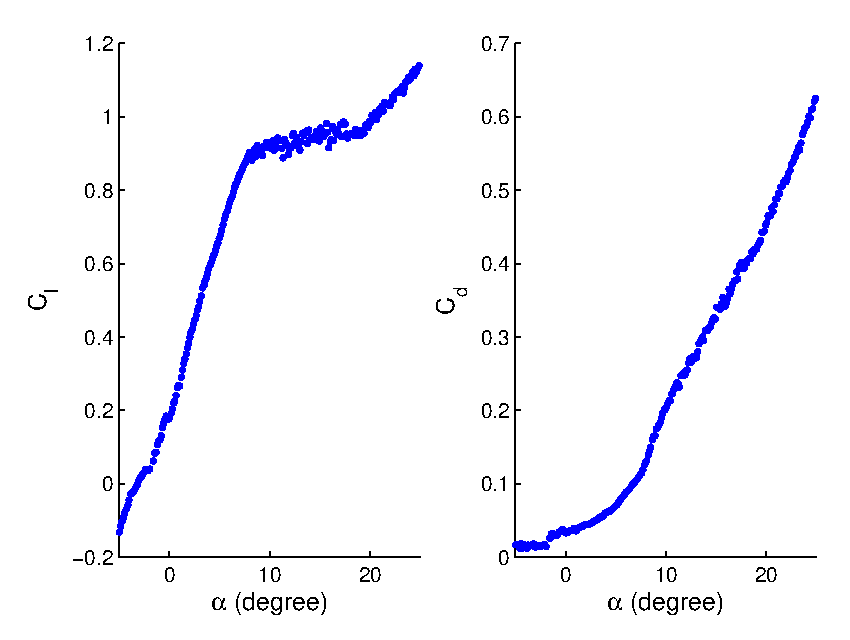
\includegraphics{./Figures/NACA0009_steady_map_Cl_Cd.eps}}
  \end{center}
  \caption{Lift and drag coefficient in the quasi-steady case}
  \label{fig:QS_Cl_Cd_vs_alpha}
\end{figure}

\par Figure \ref{fig:QS_Cl_Cd_vs_alpha} shows how the aerodynamics behave for our NACA0009 airfoil.
The lift coefficient is close to a clean linear function when the flow is attached.
The separation happens around 8 degrees and the lift coefficient remains constant in the 10 to 20 degrees zone when the flow is partially separated.
At higher angle of attack the flow is totally separated and $C_l$ is once again proportional to $\alpha$ but with a different slope this time.
Even though the NACA0009 has a symmetric profile the measured lift coefficient for a angle of attack of zero is not null.
It is suspected that the sting onto which the airfoil is fixed may disturb the flow and cause this asymmetry.
Moreover this curve differs slightly from the ones found in the literature.
Once again this can be attributed to the experimental setup; other than the sting effects the couple of millimeters of clearance between the wall of the wind tunnel and the edge of the airfoil are probably to blame as they induce some 3D effects.
These gaps are necessary for to allow for the both pitching and plunging of the wing.

\par From this static map we can approximate the part where the flow is still attached (<8 degrees) by 

\begin{equation}
  \begin{array}[c]{c}
    C_l= 2 \pi \cdot \alpha + C_l0 \\
    C_d= \frac{C_l^2}{2G_{max}} + C_d0
  \end{array}
  \label{eqn:attached_Cl_and_Cd_vs_alpha}
\end{equation}

Which is remarkably close to the classical theoretical result for a 2D airfoils in a ideal inviscid attached flow.

\Subsection{State variable approximation}
When the flow is still attached the value of $x$ is 1. 
This means that we are considering the separation point to be at the trailing edge.
Similarly when the flow is totally separated the separation point is at the leading edge and $x=0$.
Since for totally separated flow the slop of the lift coefficient as a function of $\alpha$ can be approximated to about $0.4$ of the slope for the attached flow, we choose to use the following equation for the lift over the whole range of angle of attack. 

\begin{equation}
  C_l(\alpha,x)=2 \pi \cdot \alpha (0.6 x + 0.4) + C_l0
  \label{eqn:Cl_function}
\end{equation}

\par From this equation the value of $x_0$ was then adjusted so that the output of this function matches the experimental data. 
The resulting profile for $x_0(\alpha)$ can be seen in figure \ref{fig:x_0_vs_alpha}

\begin{figure}[h]
  \begin{center}
    \scalebox{0.5}
    {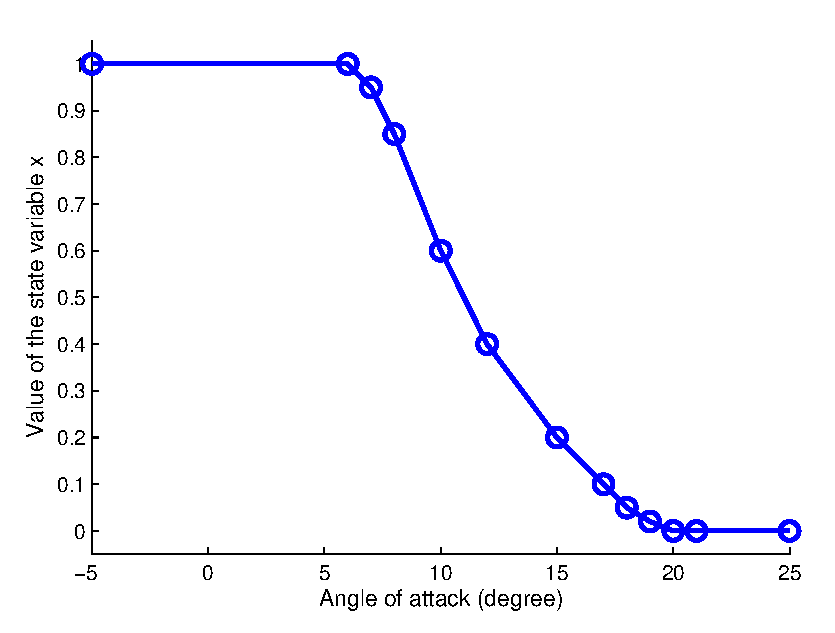
\includegraphics{./Figures/x_0_vs_alpha.eps}}
  \end{center}
  \caption{Quasi-steady profile for the state variable $x$}
  \label{fig:x_0_vs_alpha}
\end{figure}

With this profile we get a good approximation of the experimental $C_l(\alpha)$ (cf figure \ref{fig:GK_Cl_vs_alpha}) for quasi steady cases.

\begin{figure}[h]
  \begin{center}
    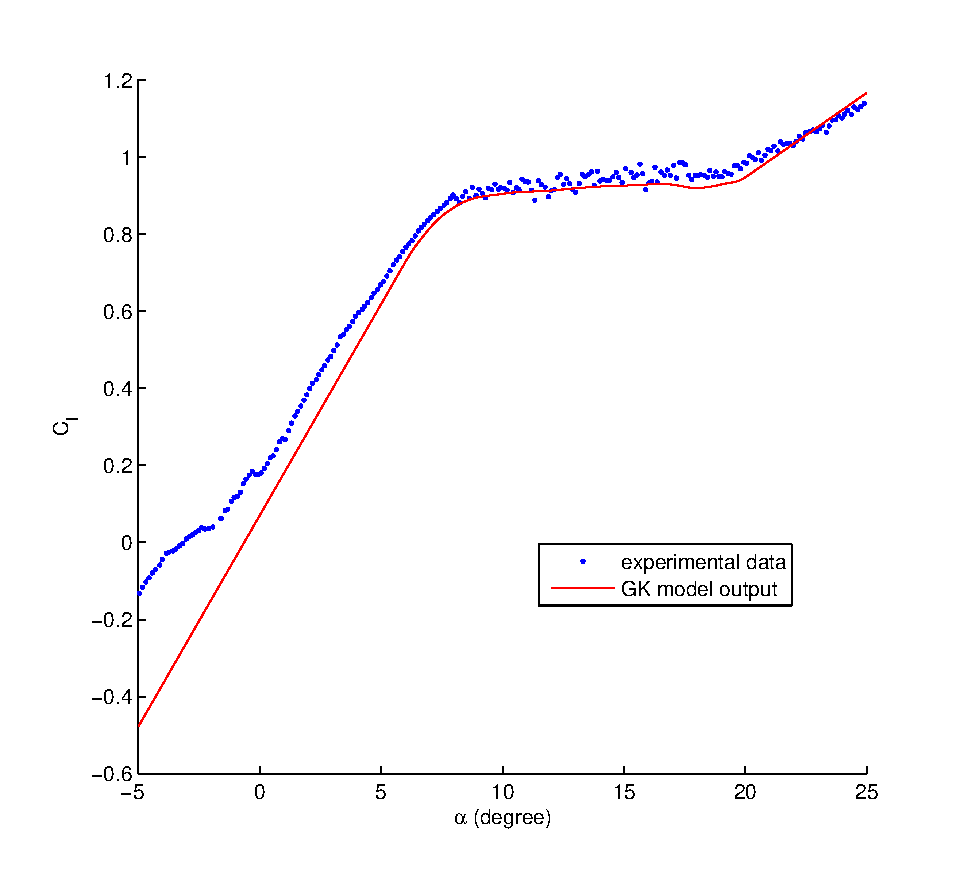
\includegraphics{./Figures/GK_cl_vs_alpha.eps}
  \end{center}
  \caption{Comparison between the experimental and model quasi-steady lift}
  \label{fig:GK_Cl_vs_alpha}
\end{figure}

\par The assumption that the drag share the same state variable as the lift is confirmed when the following equation produces similarly accurate results compared to experimental data, as seen on figure \ref{fig:GK_Cd_vs_alpha}.

\begin{equation}
  C_d(\alpha,x)= \frac{ \left( \left( 2 - x \right)C_l \right)^2 }{2 G_{max}} + C_d0
  \label{eqn:Cd_function}
\end{equation}

\begin{figure}[h]
  \begin{center}
    \scalebox{0.6}
    {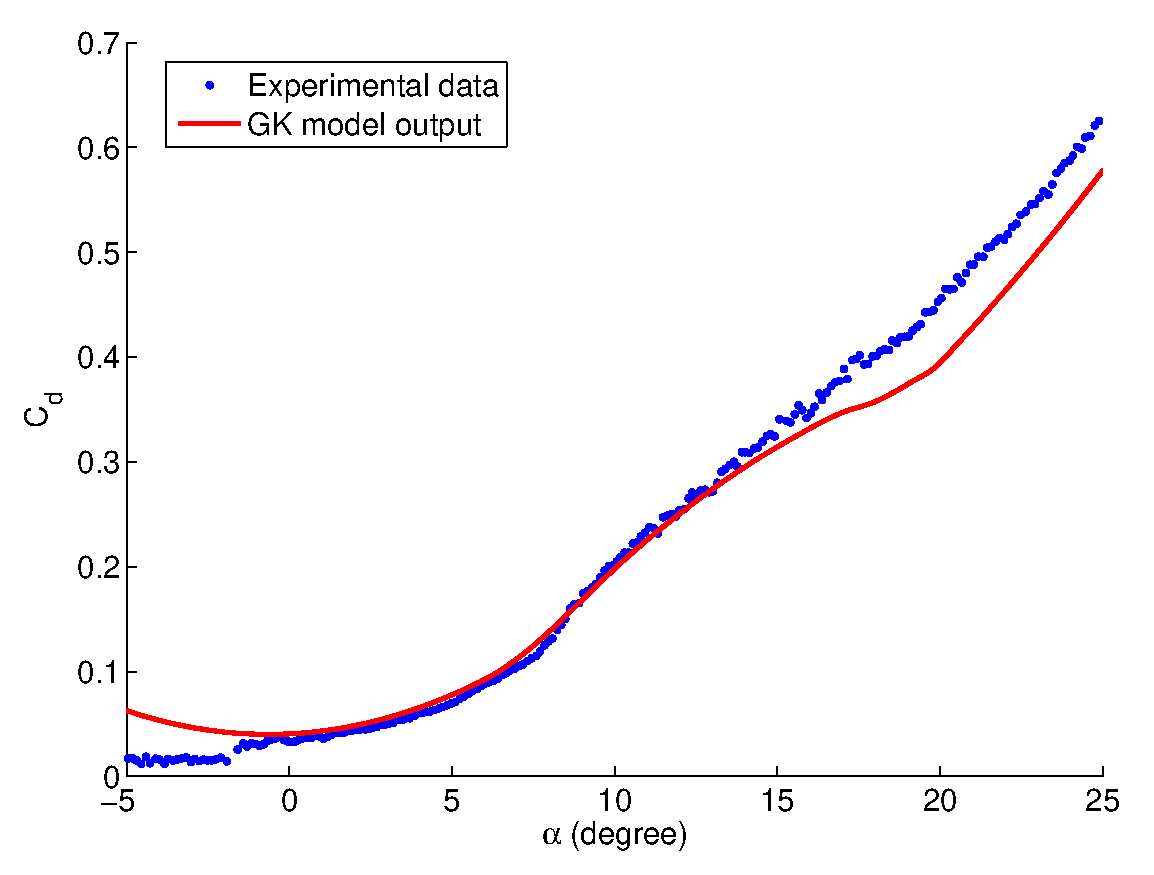
\includegraphics{./Figures/GK_cd_vs_alpha.eps}}
  \end{center}
  \caption{Comparison between the experimental and model quasi-steady drag}
  \label{fig:GK_Cd_vs_alpha}
\end{figure}

\par These two relatively simple equations shows that a physics based GK model can be implemented for both lift and drag and that they indeed depend on the same state variable.
The two time constants $\tau_1$ and $\tau_2$ will be determined in the next section when the wing undergo unsteady pithing.

\Section{Model validation}

\par While the ability to predict lift and drag based on separation can be useful, the real strength of the GK model resides in its ability to work on unsteady cases.
The first step is to determine the 2 $\tau$ time constants. 
To do that a series of pitching cases are performed. 
The pitching inputs are the following

\begin{equation}
  \alpha\left( t \right)= A \sin \left( 2 \pi \frac{t}{f} \right) + \alpha_0
  \label{eqn:pitch_input}
\end{equation}

With $A=2^\circ$ and $\alpha_0=12^\circ$.
The frequency $f$ is set to 0.25, 0.5, 1 and 2 Hz (respectively K of 0.064, 0.128, 0.257 and 0.513)

\begin{figure}[h]
  \begin{center}
    \scalebox{0.6}  
    {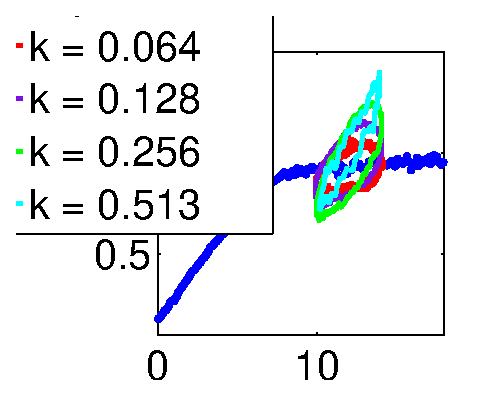
\includegraphics{./Figures/Pitching_allcases_CL_12_amp_2.eps}}
  \end{center}
  \caption{Unsteady effects of sinusoidal pitching on the lift}
  \label{fig:Pitching_allcases_Cl}
\end{figure}


% put both sinusoidal and ``random'' motion
% Also try a non dimensional validation

\par This model is producing accurate results that account for both the dynamic effects and the flow separation.
Moreover the procedure is light enough to be implemented into the optimization algorithm without increasing too much the computation cost.

%servo drive and stuff
\Chapter{Trajectory optimization with the unsteady model}
\Section{Implementation in the energy extraction algorithm}

\par As seen in the previous chapter the optimization process for the energy extraction trajectory only requires a way to calculate the relationship between the lift and drag coefficient.
Since in our case these 2 variables depend only on the angle of attack and its change rate over time, it is fairly easy to implement it into the algorithm.
However the non dimensional time constant are different, the energy extraction one consider the optimal glide speed and the gravity acceleration whereas the one used for the GK model uses the flight speed and the chord length.

\Subsection{Relation between the different time scales}
As said before the time scale used in the two models are different.
To solve this issue the ratio of the two time constants are plotted (see figure \ref{fig:T_t+_ratio}) for a wide variety of flying objects.

\begin{equation}
  \frac{T}{t+}=\frac{V_{opt}}{g} \cdot \frac{U}{c}
  \label{eqn:T_t+}
\end{equation}

Or if the aircraft flies near its optimal glide speed

\begin{equation}
  \frac{T}{t+}=\frac{V_{opt}^2}{g \cdot c}
  \label{eqn:T_t+_ratio}
\end{equation}

This ratio happens to be the Froude number.


\begin{figure}[ht]
  \begin{center}
    %\includegraphics{<+file+>}
  \end{center}
  \caption{T to t+ ratio for divers flying objects}
  \label{fig:T_t+_ratio}
\end{figure}

\par It is interesting to notice that this ratio is in the same order of magnitude for all these objects.
The value of 90 is chosen as a default for this ratio as it represent a good average of the data compiled.


\par Another issue is that the GK model is dependent on the initial value of the state variable $x$.
The initial value of $x$ is taken as the quasi-steady value.
To minimize the effect of the transition from quasi-steady to unsteady flow at the beginning of the maneuver, the cycle is simulated twice and then only the second cycle is considered.
This is possible to do since the conditions applied on the trajectory constrain the initial and final angle of attack and pitch rate to be the same.


\Subsection{Expected effects of considering unsteady aerodynamics on the optimal trajectory}
Unsteady aerodynamics allows access to new areas on the $C_l$ vs $\alpha$ map as well as on the lift to drag ratio map.
This effects on the lift and drag characteristics that will influence the optimization process if the pitching rate is fast enough to trigger them.
The effects on the lift can divided into two categories.

\par The first one is the time lag for the flow separation. 
If the airfoil is pitched up fast enough the flow doesn't have the time to separate and high values of Cl can be attained.
%Since during a typical gust negative and positive values are needed for the lift we can assume that the flow will reattach when the angle of attack is close to zero.
If the flow separates then behaviors like the one we saw in the periodic pitching around 12 degrees (see figure \ref{fig:Pitching_allcases_Cl_12}) will be seen.

\par The second effect is seen when high pitch rates are present.
In these cases the $\alpha - \tau_2 \dot{\alpha}$ term in the state variable equation \ref{eqn:state_variable} starts to get influenced by the $\dot{\alpha}$ term. 
For example for a 4 degrees amplitude sinusoidal pitching around a mean angle of attack of zero at a frequency of $k=0.5$ will produce unsteady effects as seen on the following figures \ref{fig:alpha_dalpha_vs_t} and \ref{fig:x_fast_pitching}.

\begin{figure}[h]
  \centering
  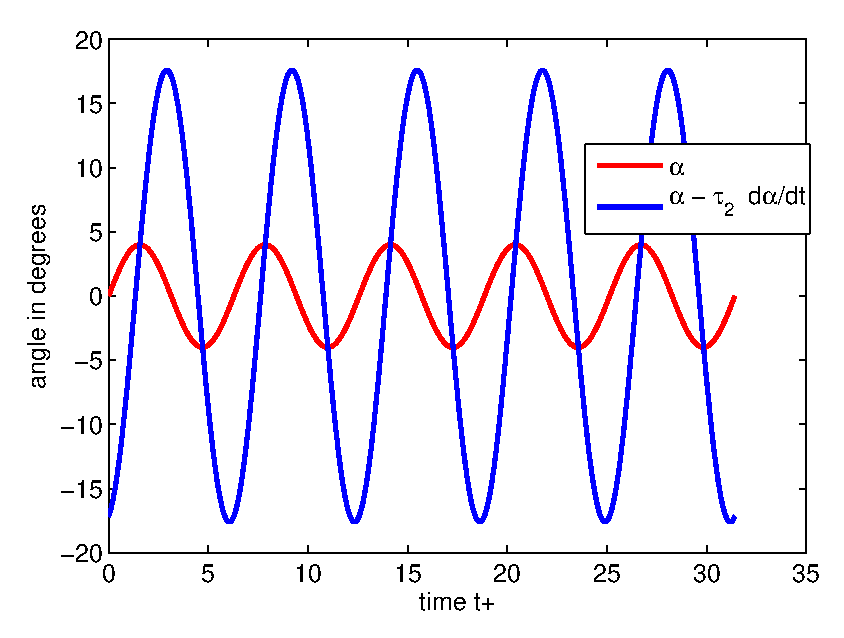
\includegraphics{./Figures/alpha_dalpha_sin_amp=4_k=0p5.eps}
  \caption{Effects of $\tau_2 \dot{\alpha}$ for high pitching rate}
  \label{fig:alpha_dalpha_vs_t}
\end{figure}


\begin{figure}[h]
  \centering
  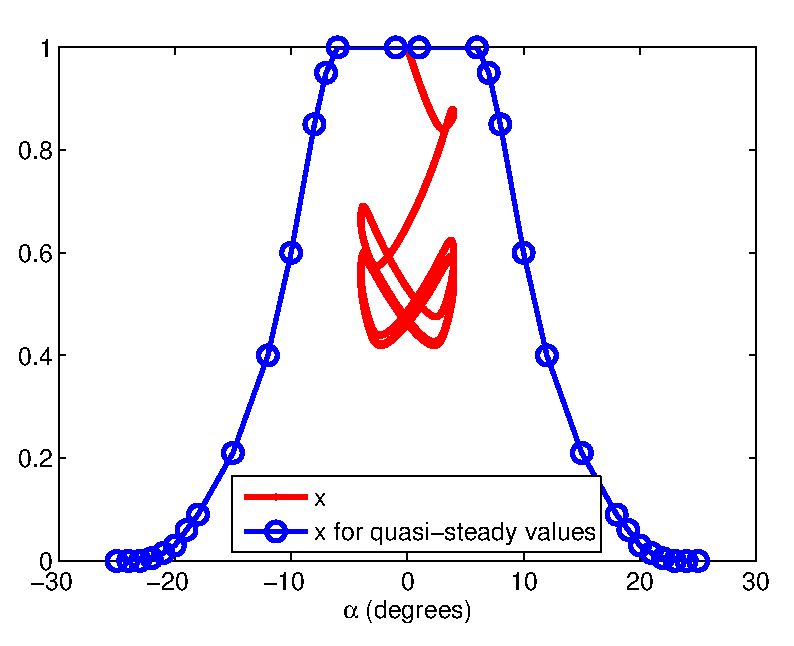
\includegraphics{./Figures/x_sin_amp=4_k=0p5.eps}
  \caption{State variable during fast sinusoidal pitching}
  \label{fig:x_fast_pitching}
\end{figure}

\par The state variable value starts at the quasi-steady value (as designed in the algorithm implementation) but after a couple of cycles it orbits close to an average value that would correspond to separated flows in a quasi-steady case.
This also leads to lower lift overall (see figure \ref{fig:Cl_fast_pitching}) since the value of x is smaller.

\begin{figure}[h]
  \centering
  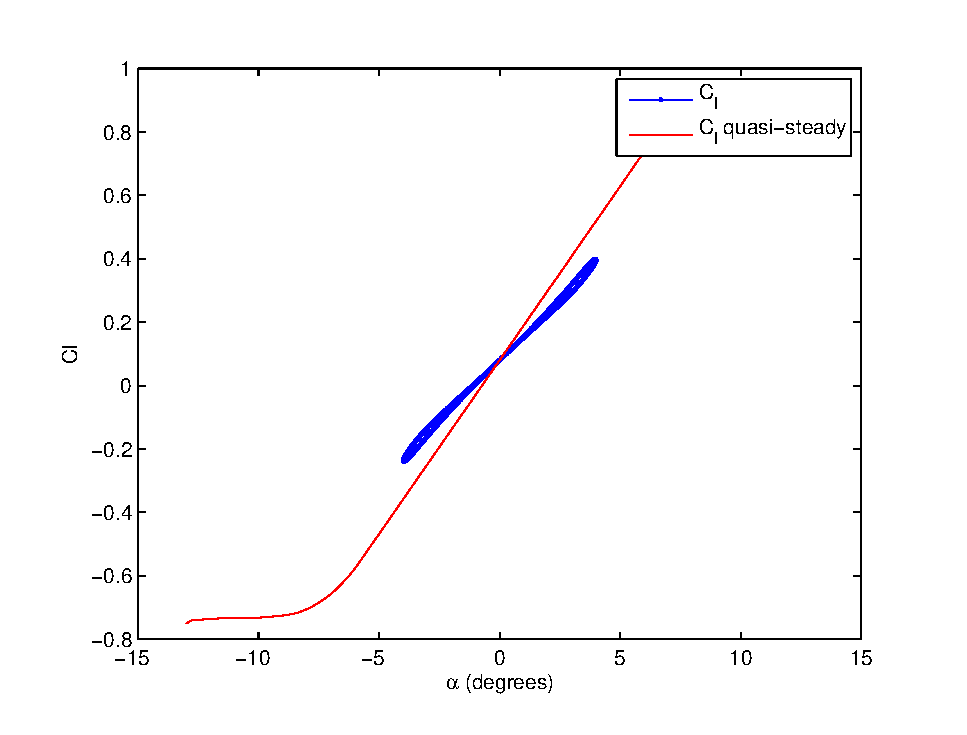
\includegraphics{./Figures/Cl_vs_alpha_amp=4_k=0p5.eps}
  \caption{$C_l$ is decreased compared to quasi-steady values for high pitching rate maneuvers (the transient part has been removed for clarity)}
  \label{fig:Cl_fast_pitching}
\end{figure}



\par If the exact same constraints are used for optimization the problem illustrated by figure \ref{fig:unlimited_alpha_dot}.	

\begin{figure}[h]
  \begin{center}
  
<++>%\includegraphics{<+file+>}
\end{center}
  \caption{Optimization for vertical wind gusts with the same constraints as the previous cases}
  \label{fig:unlimited_alpha_dot}
\end{figure}

The issue is that the in order to reach the favorable high lift regions the algorithm produces a 

%Since the lift to drag ratio of the NACA0009 is about 10 (compared to 13 for the notional UAV) direct comparisons with the results presented in part \ref{sec:results_QS} are impossible.
\Subsection{The ``staircase'' optimization issue}
All these effects dependent on the pitch rate add a lot of complexity to the optimization problem.
One of the biggest is that to keep a reasonably low execution time for the optimization the number of points has to be kept relatively low (less than a hundred).
Such discretization of the interval can cause issues in the discreet integration parts of the algorithm.
It seems that for most optimization cases this effect is avoided.

\par However the results of the of optimization for short gusts ($0.2<T_g<0.5$) sometime shows a ``staircase'' pattern in the angle of attack.

\begin{figure}[h]
  \centering
  %\includegraphics{<+file+>}
  \caption{Staircase pattern seen for XXXX wind gust with $T_g=XX$}
  \label{fig:staircase_case}
\end{figure}

\par In those cases the algorithm seems to try to ``game'' the GK model with this jerky pitch motion.
Our theory is that this jerky motion avoids the decrease of the lift coefficient caused by high pitch rates by doing those for only short amount of time.
These spikes in the pitch rate are too short to be able to influence the low pass equation regulating the value of $x$.





\Section{A closer look at the high performing short gusts}

\begin{figure}[h]
  \begin{center}
  \scalebox{1.0}{
    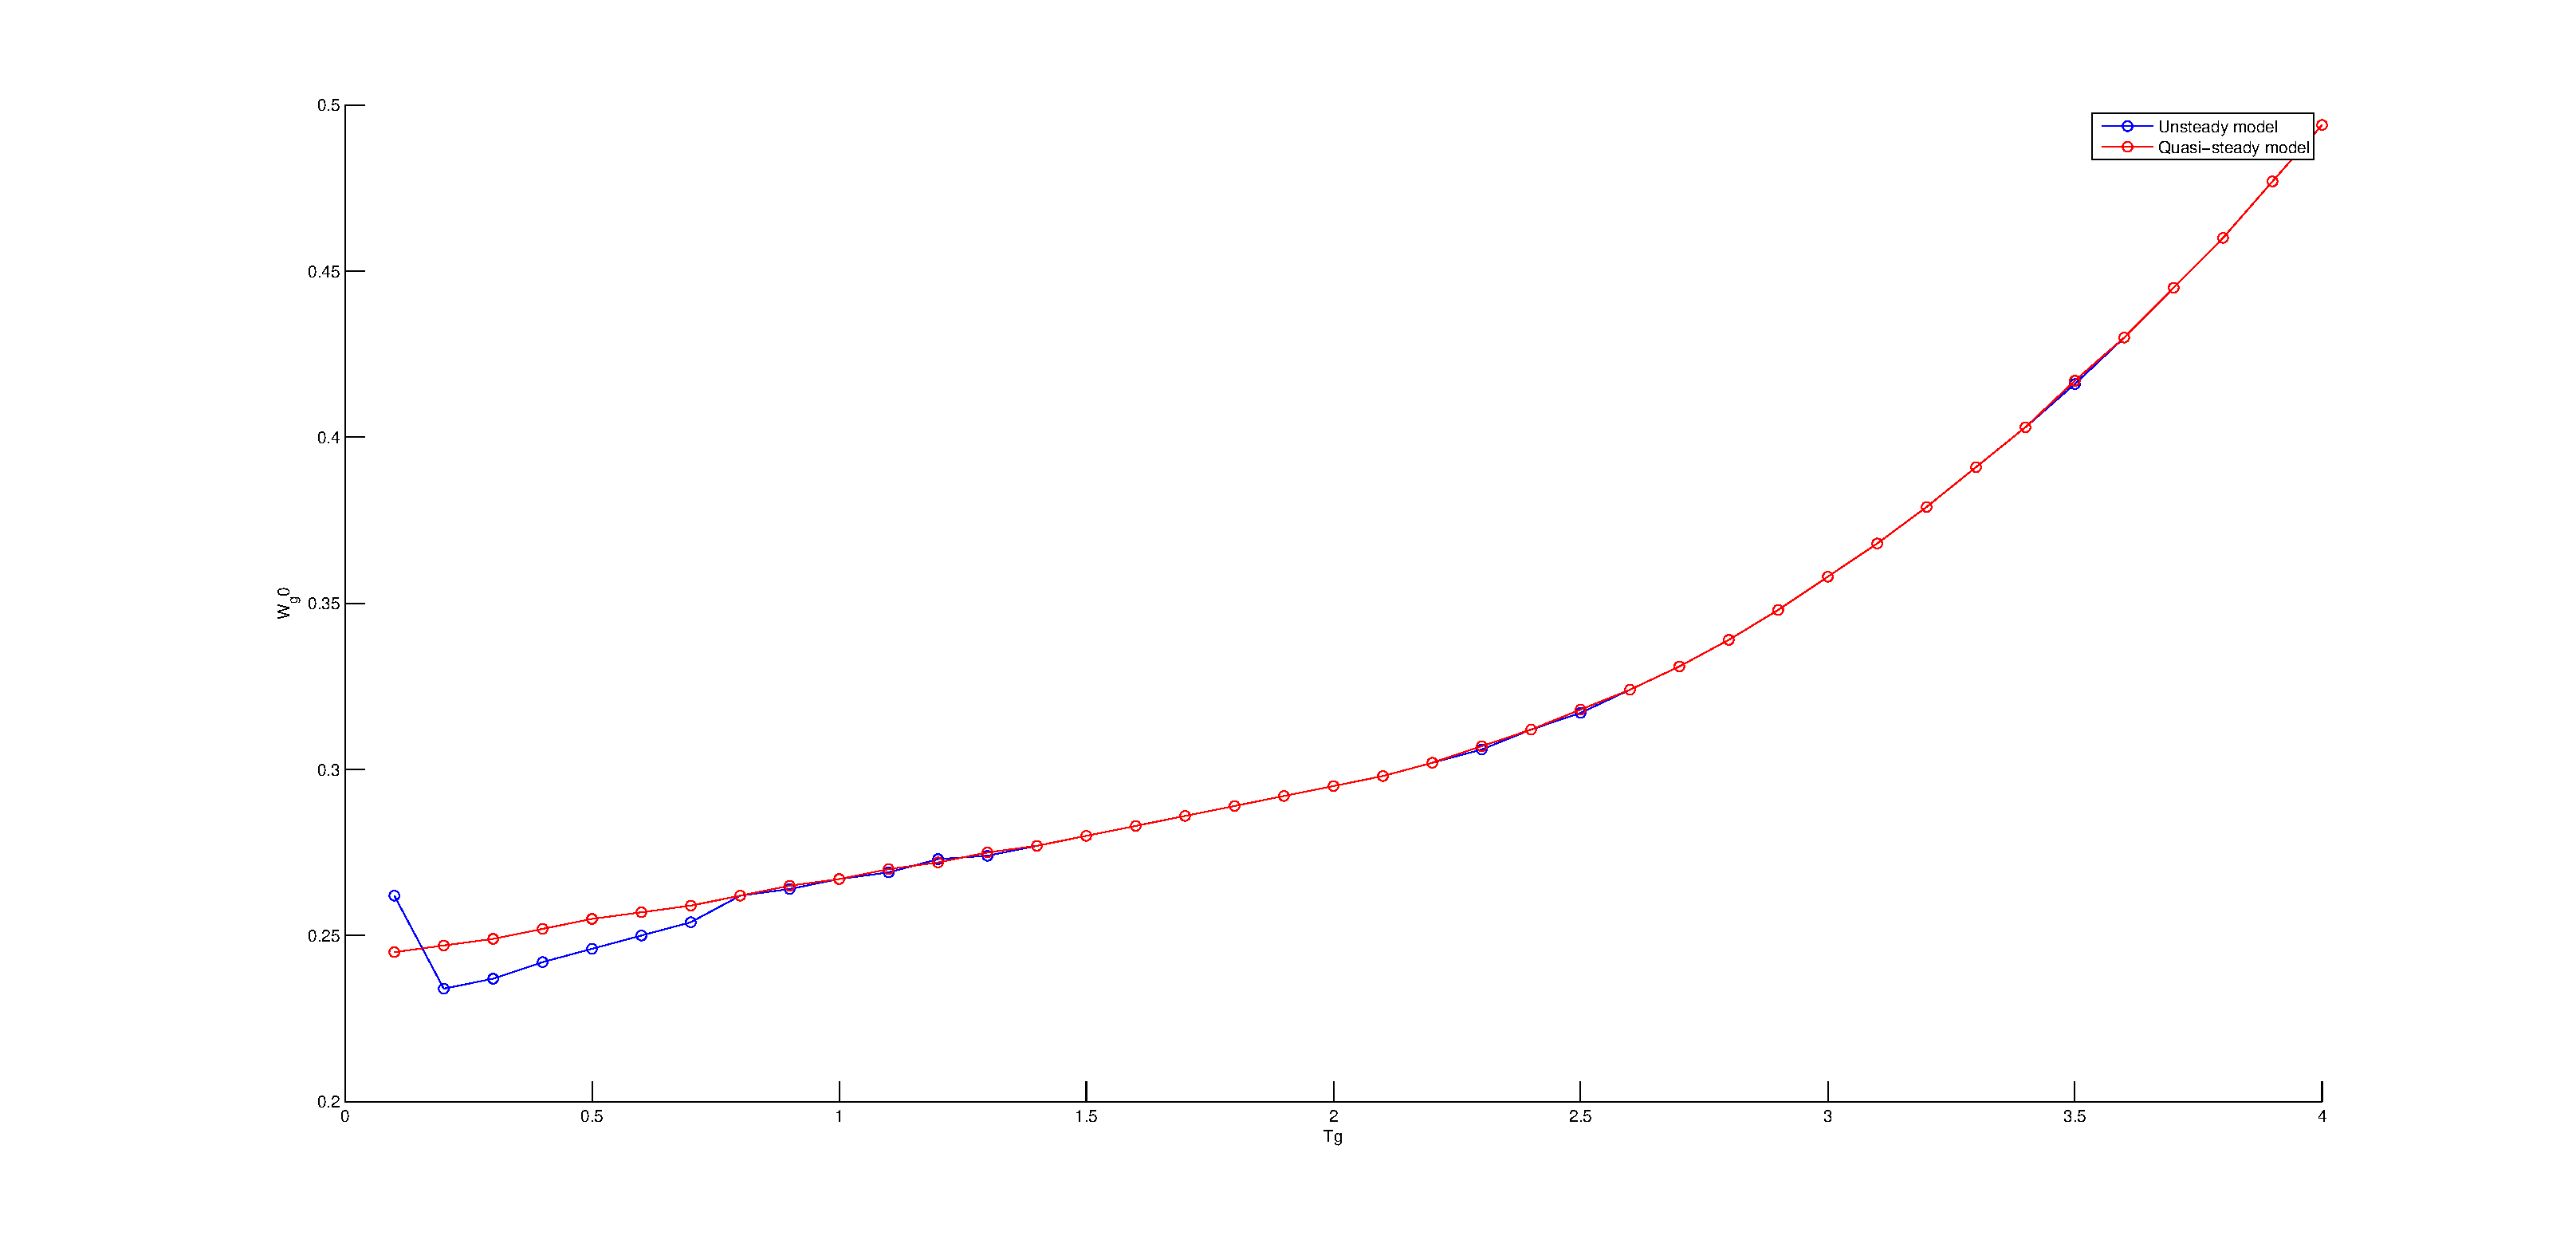
\includegraphics{./Figures/Wg_vs_TG_windtype=3_alphamax=12_nodalphalimit.eps}}
  \end{center}
  \caption{Performance difference between quasi-steady and unsteady model for combined gusts}
  \label{fig:WG_vs_TG_wt=3}
\end{figure}


\begin{figure}[h]
  \centering
  \scalebox{1.0}{
    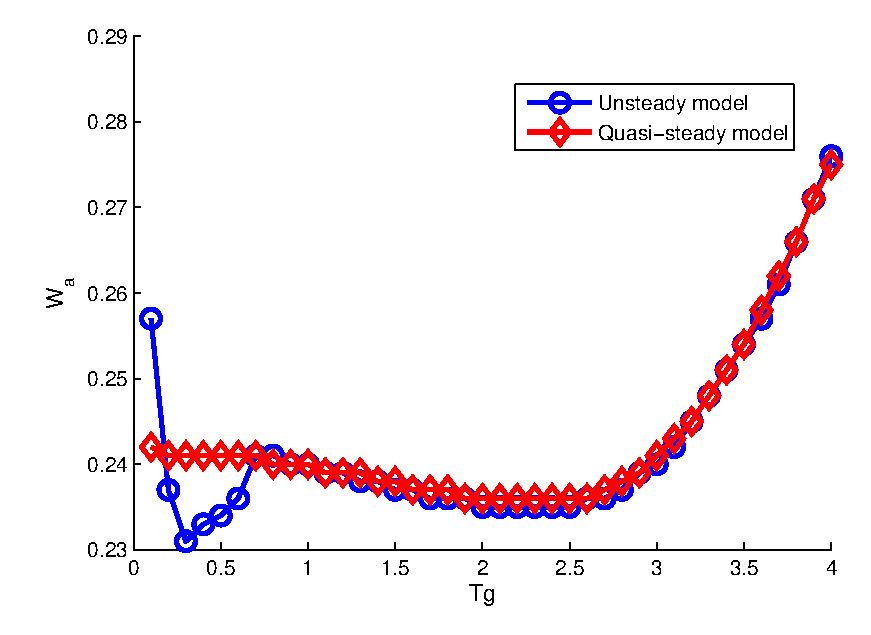
\includegraphics{./Figures/Wg_vs_TG_windtype=1_alphamax=12_nodalphalimit.eps}}
  \caption{Performance difference between quasi-steady and unsteady model for vertical gusts}
  \label{fig:WG_vs_TG_wt=1}
\end{figure}

\par The difference between the quasi-steady model and the unsteady one only appears close for $Tg<0.7$.
This result is reassuring as it confirm that for long gusts ($Tg>0.7$ or $k<0.05$) the two model are equivalent.
We can confirm that there is no unsteady effects active by looking at the $C_l$ versus $\alpha$ curve compared to the quasi-steady map, or even better $G$ the lift to drag ratio.
On figure \ref{fig:G_vs_alpha_wt=1_Tg=1_GK.eps} you can see that the lift to drag ratio for $T_g=1$ is following the quasi-steady values.

\begin{figure}[h]
  \centering
  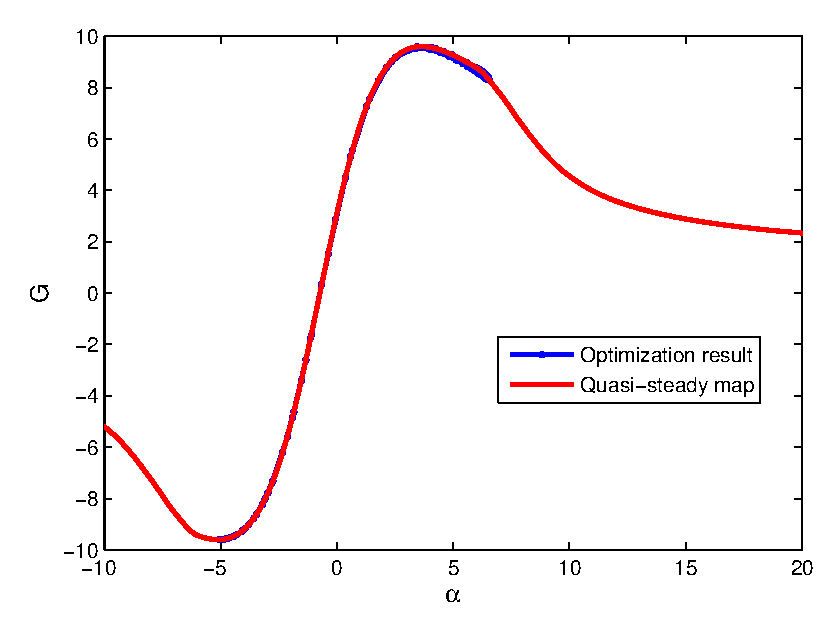
\includegraphics{./Figures/G_vs_alpha_wt=1_Tg=1_GK.eps}
  \caption{Lift to drag ratio for the unsteady model, vertical wind gust and gust duration of 1T}
  \label{fig:G_vs_alpha_wt=1_Tg=1_GK.eps}
\end{figure}

\par However for shorter gusts the results are more interesting.
We can see that for shorter gusts ($T_g<0.7$) the performances are better with the GK model than with the quasi-steady model.
This is true for both vertical and combined wind gusts which seems to indicate that this is due to the unsteady effects starting to be significant at this frequency.

\FloatBarrier

\par Looking more precisely at the results around $T_G=0.3$ let's try to highlight thee differences between the quasi-steady and the unsteady model.
First we can look at the optimization parameter $\alpha$ for both vertical and combined gusts.

\begin{figure}[h]
  \centering
  \scalebox{1.0}{
    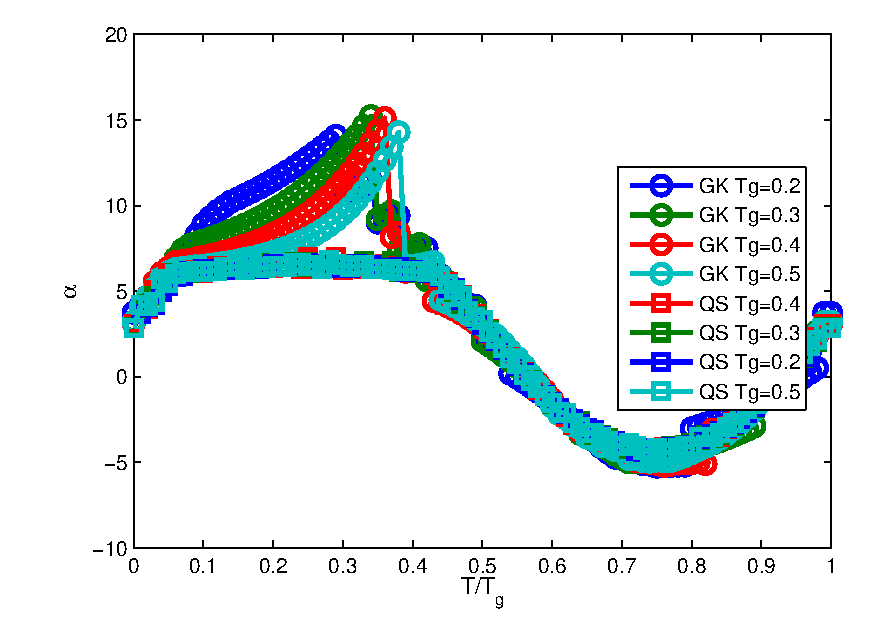
\includegraphics{./Figures/alpha_vs_Tg_wt1.eps}}
  \caption{Angle of attack for short vertical gusts with the quasi-steady (QS) and unsteady (GK) model}
  \label{fig:alpha_vs_Tg_wt1}
\end{figure}

\begin{figure}[h]
  \centering
  \scalebox{1.0}{
    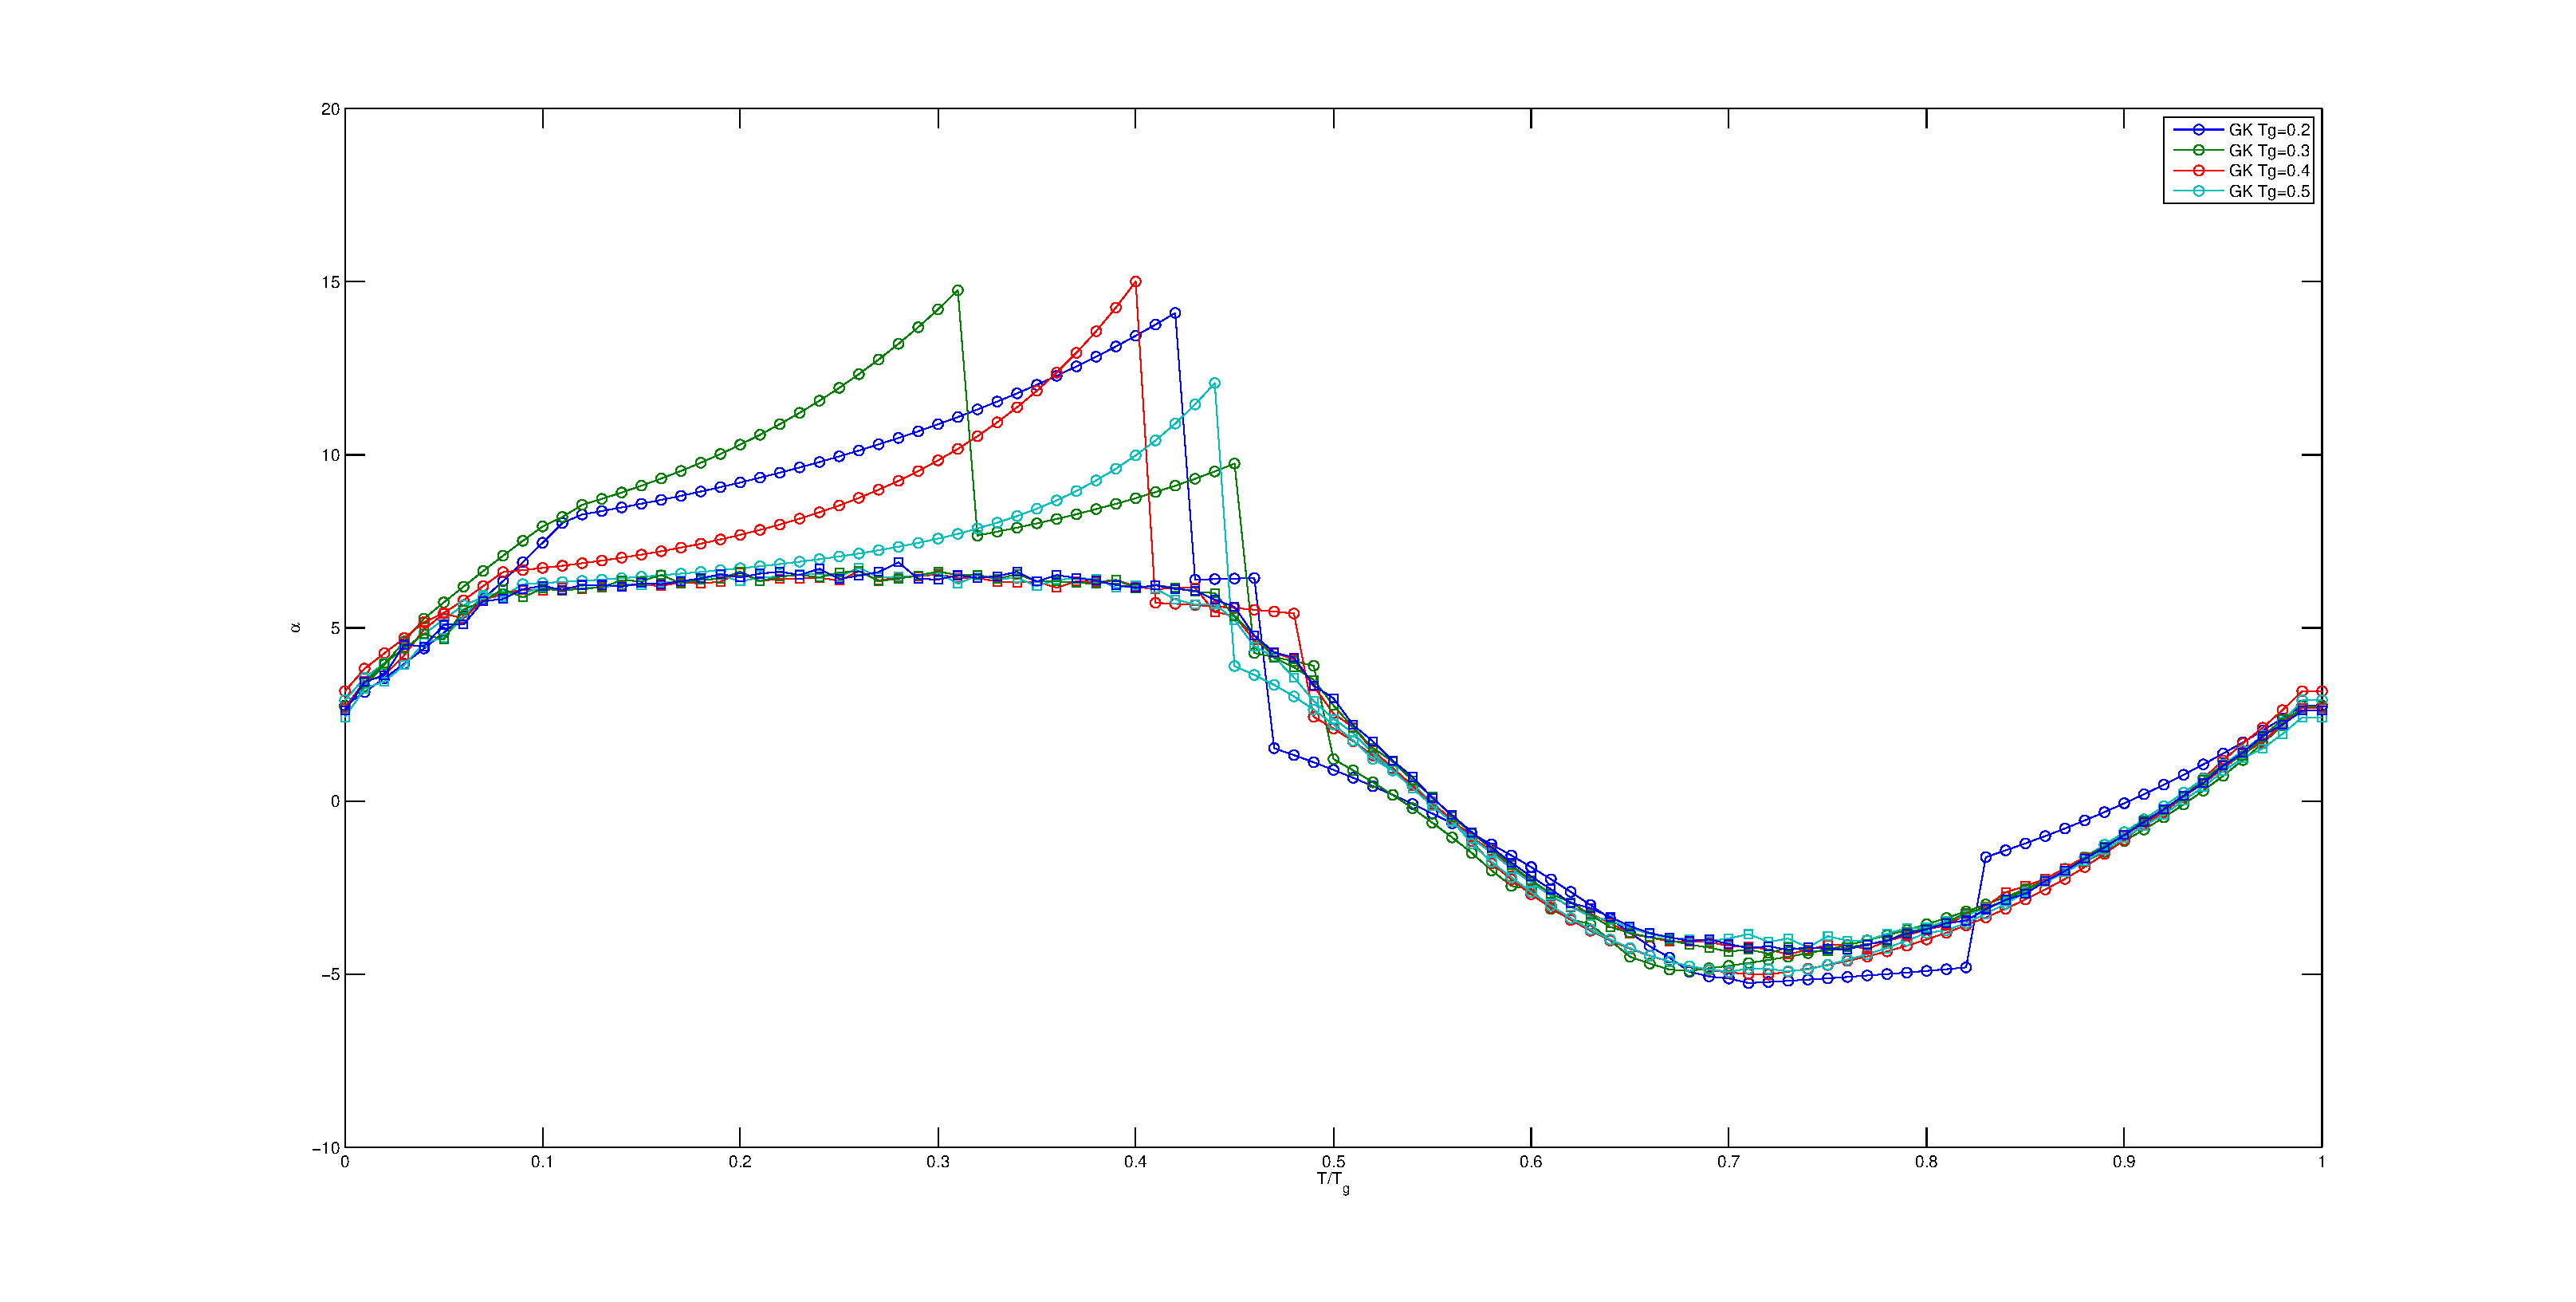
\includegraphics{./Figures/alpha_vs_Tg_wt3.eps}}
  \caption{Angle of attack for short combined gusts with the quasi-steady (QS) and unsteady (GK) model}
  \label{fig:alpha_vs_Tg_wt3}
\end{figure}

\par It is immediately apparent that the main difference is in the high angle of attack area.
Alpha increases exponentially before a sharp decrease happens around 30 to 40\% of the gust duration.
The angle of attack then falls back to the quasi-steady values.

\FloatBarrier

\par To understand what happens to the lift when such a maneuver is performed we have to refer to the lift coefficient versus angle of attack plot.

\begin{figure}[h]
  \centering
  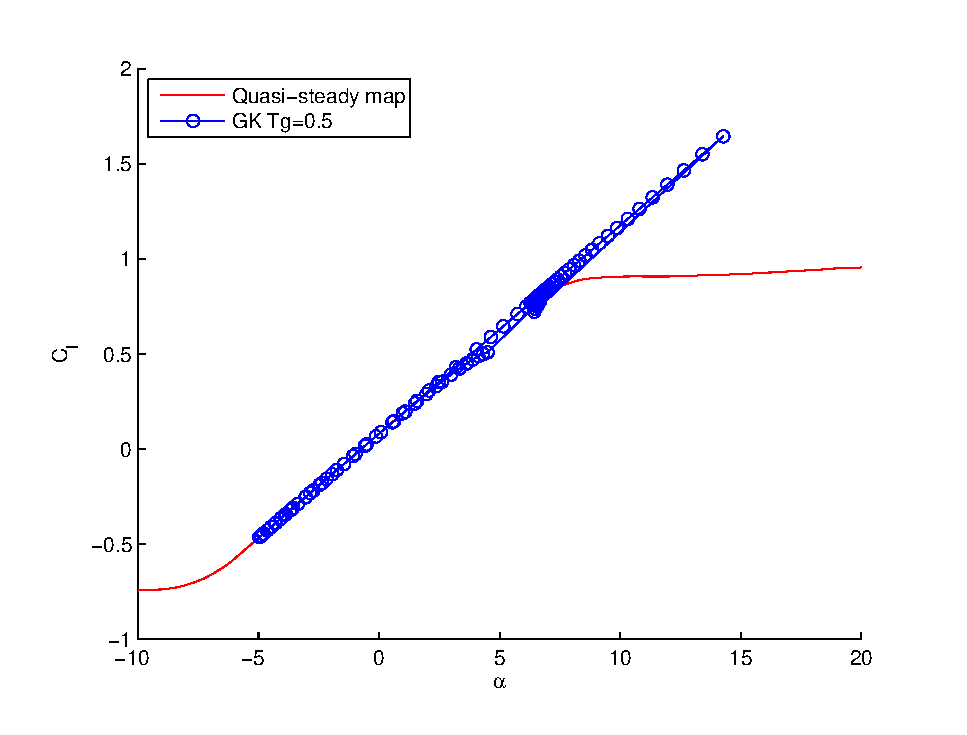
\includegraphics{./Figures/Cl_vs_alpha_wt=1_tg=0p5_alphamax=20.eps}
  \caption{Lift coefficient versus angle of attack for 0.5T long vertical wind gusts with the unsteady model}
  \label{fig:Cl_vs_alpha_short_gust_unsteady}
\end{figure}
\FloatBarrier

\par Figure \ref{fig:Cl_vs_alpha_short_gust_unsteady} illustrate perfectly the effects of the unsteady aerodynamic model and the difference with the quasi-steady model.
The spiking in angle of attack allows the flow to remain attached to the airfoil and let the lift coefficient reach values for superior to what the quasi-steady (red curve) model would ever permit.
Sharply decreasing the angle of attack at the end of this maneuver means that the flow doesn't have time to separate.
Similar results are observed for vertical and horizontal gusts in the $T_g=0.2$ to $0.7$ region.



\Section{Bad performances at $T_g\leq0.1$}

\par As seen on figures \ref{fig:WG_vs_TG_wt=3} and \ref{fig:WG_vs_TG_wt=1} while the unsteady model optimizations are showing a more efficient energy extraction than the quasi-steady for $0.2 \leq T_g \leq 0.7$ it is not the case at $T_g=0.1$. 


\Section{Limitations of the unsteady GK model}

\Subsection{Considering the gusting and plunging component}
One of the major thing this optimization misses are the unsteady effects due to gusting and plunging.
In our case we have major gusts present at the same time as the pitching motion.
While the speed of the UAV changes too, the relative wind amplitude is in the order of 20\%.
We know that gusts as gentle as 5\% of the free stream speed can have huge influence on the lift characteristics and that the lift response to such gusts depends heavily on the frequency of the gusts.
The same can be said for the plunging motion.

\par While this variations are pretty wild it is suspected that they are caused by the same kind of mechanism as the lift variations caused by pitch angle changes.
With that in mind there is a fairly high probability that the resulting mechanism could be described by a model inspired by the GK model.
It is very likely that the state variable for such a model would be tied in some way to the state variable presented in this thesis.
If $x$ could be expressed as a function of $\alpha$, $\dot{\alpha}$ and $\dot{u}$ (for example), this model could be applicable to a whole new range of situations.



\Subsection{Moment of inertia considerations}



\Chapter{CONCLUSION}

\Section{Low order model for unsteady flow}

\par The Goman and Khrabrov model shows good agreement in both shape and magnitude for the lift and drag of a pitching airfoil in a wide range of conditions.
It is fast and light and can be adjusted to a new airfoil (or even a whole aircraft) without requiring extensive experimental studies.
In fact in theory only a static map and one unsteady case should be enough to obtain the whole model.

\par The work in this thesis has proven that the drag can also be easily modeled and there is little doubt that the moment coefficient $C_m$ could be modeled too.

\par Implementing this model is simple enough that it can be used in computationally heavy applications such as optimization problems or real time applications.
It is however non-linear and as such isn't easily invertible or analyzable with traditional control system methods.

\Section{Energy extraction optimization}

\par From the results presented in this thesis it can be seen that energy extraction can be performed for complex temporal wind gusts with vertical and horizontal components.
In these gusts overall neutral energy trajectories are possible and require less and less wind gust amplitude the shorter the gust is.
For short gust ($T_g \le 3$) high angles of attack are needed for maximum performance, which can lead to flow separation.

\par The introduction of an unsteady aerodynamic model is possible and proves necessary when gusts are very short ($T_g \le 0.7$ or $k \ge 0.05)$).
At this point unsteady effects such as lag in the flow separation can be observed and even taken advantage of.
While the maneuvers required to obtain such trajectories are unlikely to be realistically done on aircrafts, these results could be exploited in vertical wind turbine pitch optimization for example.
The results for gusts shorter than $T_g=0.2$ ($k=0.175$) are less obvious to interpret and will require further study, perhaps with a problem more representative of the system operating at such frequencies.

\par While these results shows the optimal trajectory found by the algorithm it is important to keep in mind that the algorithm optimize the trajectory globally over the whole period.
This means that it can take preemptive actions because it ``knows'' what will happen later in time.
A real controller flying in an environment where the wind gust shape can't be predicted would not be able to reach the same energy extraction performances.

\Section{Possible improvements and additional work}

\par One of the weakness of the optimization with the GK model is that it does not account for the unsteady effects due to the surging and gusting components of the relative wind.
I believe that the GK model could be modified to include these effects but a complete experimental campaign would be needed.

\par The ``staircase'' effect described in section \ref{sub:staircase} could be mitigated by introducing a more realistic model for the aircraft dynamics that include the moment of inertia.
Going even further, a basic elevator model could be implemented.

\par Finally replacing the temporal wind profile by a spatial one would allow for the use of more realistic and complex wind fields.




\clearpage


%
% APPENDIX
%

% Do the settings of appendices with \appendix command
\appendix

% Then create each appendix using
% \Appendix{title_of_appendix} command

\Appendix{Goman Khrabrov model Matlab\textsuperscript{\textregistered} implementation} \label{ch:GK_code}
\lstinputlisting{./NACA0009_GK.m}
%\moretox




%
% BIBLIOGRAPHY
%
% you have two options: 1) create bibliography manually,
% 2) create bibliography automatically. See BibliographyHelp.pdf file for details.


\bibliographystyle{plain}
\bibliography{mybib}


\end{document}  % end of document
